\chapter{User Documentation}

In this chapter, the user will get a general introduction to the usage of the thesis template and will be enabled to start with his work.
Further information is given in the subsequent chapters.
But don't be afraid, there is no need for you to read through all of it before starting your work.
Instead, you might find it useful to just look at the table of contents and decide which sections you need to look at later when looking for a solution to a problem.


\section{Introduction}\label{sec:user-documentation:introduction}

\subsection{Target Users}\label{sec:user-documentation:target-users}

Writing a good thesis can be cumbersome if you have never done it before.
Even for experienced researches having published a sum of papers, writing up a thesis is not the same.
Without underestimating the complexity of writing a thesis, it is cumbersome to get it all nicely wrapped up and in layout that is consistent from start to end.
This thesis template tries to fill the gap between content and layout by providing you with certain commonly used packages and styles set to have a consistent layout that you don't have to bother about maintaining.


\subsection{Features of the Class}\label{sec:user-documentation:features}

With this thesis template you write a simple, nicely typeset thesis without the hassle of needing to configure it such that it suits the needs of your department (it should have applied all the necessary style guidelines already).


\subsection{How to Get Started}\label{sec:user-documentation:get-started}

In order to get your thesis started, there is a few things necessary to set up.
One of them being obviously the choice of a good typewriting environment.
The list out there for writing your thesis is longer than it should be so we will just briefly mention some of the most common editors (both IDE and simple text editors).
Choose by your own needs


\subsubsection{Configure Editor and System Settings}\label{sec:user-documentation:configure-system}

You must choose a \LaTeX distribution and an editor.
For a list of editors, please refer to or the following list (which is only an excerpt from the SO page).
We prefer TeXstudio even though its implementation of using some keys can be cumbersome at times.

\paragraph{Emacs with AUCTeX}
\begin{itemize}
    \item \textit{Platforms:} Windows, Mac (incl. Aquamacs fork), Unix
    \item \textit{License:} Free software (GPL)
    \item \textit{Languages:} de, dk, fr, is, it, jp, nl, pl, se, sk are supported by AUCTeX language styles
    \item \textit{Unicode:} Yes, from Emacs 23, characters are represented using Unicode
    \item \textit{RTL/bidirectional support:} From Emacs 24, through bidi-mode
    \item \textit{\% !TEX directives:} No, but has several realizations of file local variables
    \item \textit{Syntax highlighting:} Yes, customisable through customize and Elisp
    \item \textit{Code completion:} Yes, via Emacs Predictive Completion, which supports AUCTeX without further configuration
    \item \textit{Code folding:} Yes
    \item \textit{Spell checking:} Yes
    \item \textit{SyncTeX:} Yes
    \item \textit{Built-in output viewer:} Yes
    \item \textit{Project management:} org-mode, reftex-mode, speedbar
\end{itemize}

\paragraph{Vim with LaTeX-suite}
\begin{itemize}
    \item \textit{Platforms:} Windows, Mac, Linux and others
    \item \textit{License:} Open Source Charityware
    \item \textit{Languages:} ?
    \item \textit{Unicode:} Yes
    \item \textit{RTL/bidi support:} partially
    \item \textit{\% !TEX directives:} No, but has modelines
    \item \textit{Syntax Highlighting:} Yes, customizable
    \item \textit{Code Completion:} Yes (using Omni Completion, extendable with SnipMate plugin)
    \item \textit{Code Folding:} Yes
    \item \textit{Spell Checking:} Yes
    \item \textit{SyncTeX:} Yes, see e.g. this question
    \item \textit{Built-in Output Viewer:} No
    \item \textit{Project Management:} ?
\end{itemize}

\paragraph{Texmaker}
\begin{itemize}
    \item \textit{Platforms:} Windows XP/Vista/7/8, OS X 10.5+, Linux
    \item \textit{License:} GPL license, free
    \item \textit{Languages:} cs, de, el, en, es, fa, fr, gl, hu, it, nl, pl, pt, pt (bra), ru, se, sr, zh (cn), zh (tw)
    \item \textit{Unicode:} Yes
    \item \textit{RTL/bidi:} ?
    \item \textit{\% !TEX directives:} No
    \item \textit{Syntax Highlighting:} Yes, customizable
    \item \textit{Code Completion:} Yes, customizable
    \item \textit{Code Folding:} Yes
    \item \textit{Spell Checking:} Yes
    \item \textit{SyncTeX:} Yes
    \item \textit{Built-in Output Viewer:} Yes, supports PDF
    \item \textit{Project Management:} Yes
\end{itemize}

\paragraph{TeXstudio (formerly TexMakerX)}
\begin{itemize}
    \item \textit{Platforms:} Windows XP/Vista/7, OS X, Linux, FreeBSD
    \item \textit{License:} GPL v2
    \item \textit{Languages:} cs, de, en, es, fr, hu, ja, pt\_BR, zh\_CN
    \item \textit{Unicode:} Yes
    \item \textit{RTL/bidi:} ?
    \item \textit{\% !TeX directives:} Yes
    \item \textit{Syntax Highlighting:} Yes, customizable
    \item \textit{Code Completion:} Yes, customizable and auto-customized
    \item \textit{Code Folding:} Yes
    \item \textit{Spell Checking:} Yes
    \item \textit{SyncTeX:} Yes
    \item \textit{Built-in Output Viewer:} Yes, supports PDF
    \item \textit{Project Management:} Yes
\end{itemize}

\paragraph{TeXworks}
\begin{itemize}
    \item \textit{Platforms:} Windows XP/Vista/7/8, OS X, Linux all pre-compiled plus source available
    \item \textit{License:} GPL
    \item \textit{Languages:} en, af, ar, ca, cs, de, fa, fo fr, it, ja, nl, ko, pl, pl, ru, sl, tr zh
    \item \textit{Unicode:} Yes
    \item \textit{RTL/bidi:} Yes
    \item \textit{\% !TEX directives:} Yes
    \item \textit{Syntax Highlighting:} Yes, regex-based
    \item \textit{Code Completion:} Yes, customizable based on 'known entry' list
    \item \textit{Code Folding:} No
    \item \textit{Spell Checking:} Yes, but have to install by hand
    \item \textit{SyncTeX:} Yes
    \item \textit{Built-in Output Viewer:} Yes, PDF (Poppler-based)
    \item \textit{Project Management:} No
\end{itemize}

\paragraph{TeXnicCenter}
\begin{itemize}
    \item \textit{Platforms:} Windows XP/Vista/7/8
    \item \textit{License:} Open Source
    \item \textit{Languages:} English, German, more dictionaries for spelling control downloadable
    \item \textit{Unicode:} Yes (in version 2, which was released mid-september 2013).
    \item \textit{RTL/bidi:} ?
    \item \textit{\% !TEX directives:} No
    \item \textit{Syntax Highlighting:} Yes, customizable (also background colour)
    \item \textit{Code Completion:} Yes
    \item \textit{Code Folding:} Yes
    \item \textit{Spell Checking:} Yes
    \item \textit{SyncTeX:} Yes
    \item \textit{Built-in Output Viewer:} No. You can config TeXnicCenter to use an external PDF viewer like Acrobat Reader or SumatraPDF with synchronized viewing.
    \item \textit{Project Management:} Yes
\end{itemize}

\subsubsection{Configure the Document}\label{sec:user-documentation:configure-document}

\subsubsection{Start Writing your Content}\label{sec:user-documentation:writing}


\section{Conventions, Settings, Typesetting, etc.}\label{sec:user-documentation:settings}































\chapter[The Short Title of the Chapter Showing Up in the TOC and the Page Headers]{The Very First Chapter With a Very Long Title Just to See What it Looks Like Since it Spans Multiple Lines in the ToC}


\lipsum[1]

\chapter{A Second Chapter}

\lipsum[1]

\section{A First Section}

\lipsum[1]

\subsection{A Sample Subsection}

\lipsum[1]

\subsubsection{A Sample Subsubsection}

\lipsum[1]

\paragraph{A Sample Paragraph}
\lipsum[1]

\subparagraph{A Sample Subparagraph}
\lipsum[1]


\chapter{The Main Template}

\section{Document Structure}

You are free in organizing your document, however, it is recommended that a certain order of chapters is always obeyed to. The chapters must be given in the following order

\begin{enumerate}
    \item Titlepage
    \item Titlepage in second language (in German or English if thesis written in English or German, respectively)
    \item Dedication (not needed)
    \item Copyright (not needed)
    \item Declaration of Authorship (needed only for student theses)
    \item Table of Contents
    \item List of Figures
    \item List of Tables
    \item List of Abbreviations (not needed, textual abbreviations like e.g., CDPR)
    \item List of Symbols (not needed, math symbols and alike)
    \item Acknowledgments (not needed)
    \item Abstract (with keywords)
    \item Abstract in second language (in German or English if thesis written in English or German, respectively)
    \item The main content (in \verb|\chapter|)
    \item Appendix or appendices
    \item Bibliography
\end{enumerate}

\begin{figure}
    \centering
    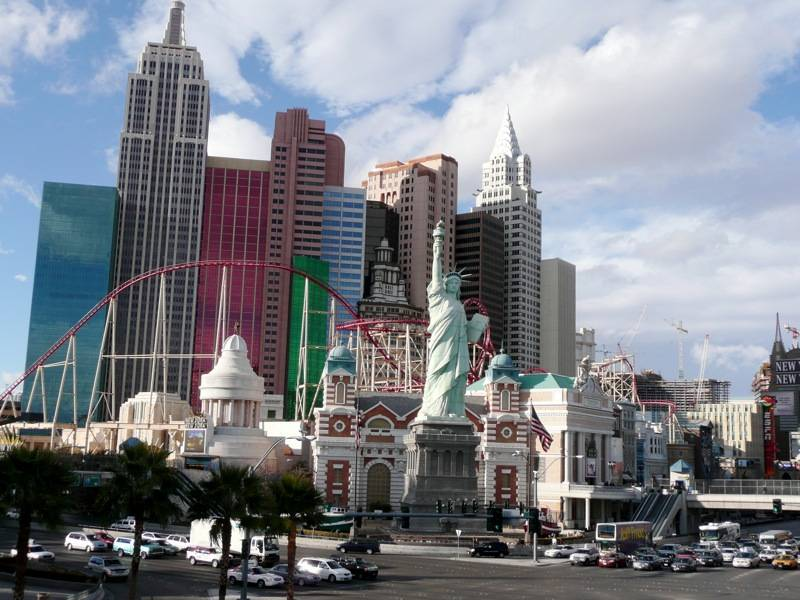
\includegraphics[width=\linewidth, keepaspectratio=true]{placeholder/800-600-1}
    \caption{A sample figure of the New York Hotel at Las Vegas, NV, USA showing the effect of a loooong looooong caption.}
    \label{fig:sample-figure}
\end{figure}

\begin{figure}
    \centering
    \begin{subfigure}[b]{0.49\textwidth}
        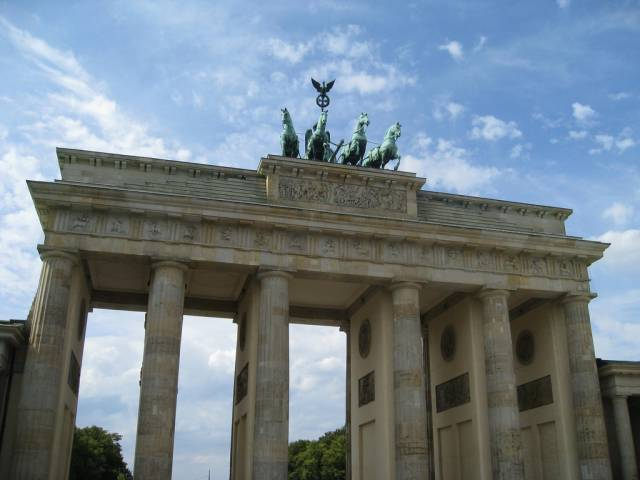
\includegraphics[width=\textwidth, keepaspectratio]{placeholder/640-480-1}
        \caption{Picture 1.}
        \label{fig:subfigures-two:1}
    \end{subfigure}
    \hfill
    \begin{subfigure}[b]{0.49\textwidth}
        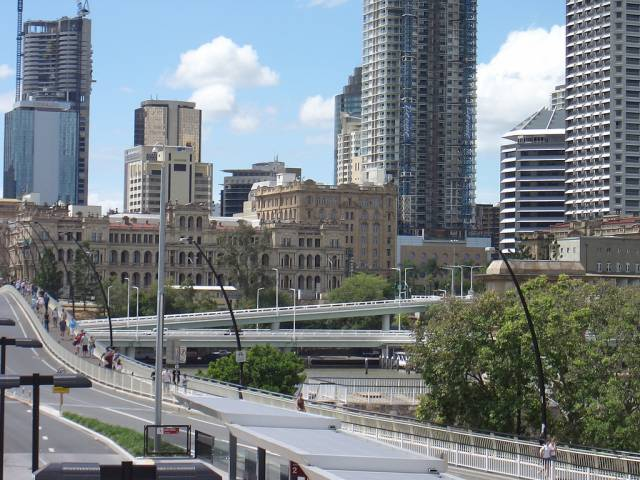
\includegraphics[width=\textwidth, keepaspectratio]{placeholder/640-480-2}
        \caption{Picture 2.}
        \label{fig:subfigures-two:2}
    \end{subfigure}
    
    \caption{Even subfigures of two figures are possible and the left one is referenced like so \subref{fig:subfigures-two:1} while the right one is referenced like so \subref{fig:subfigures-two:2}.}
    \label{fig:subfigures-two}
\end{figure}

\begin{figure}
    \centering
    \begin{subfigure}[b]{0.49\textwidth}
        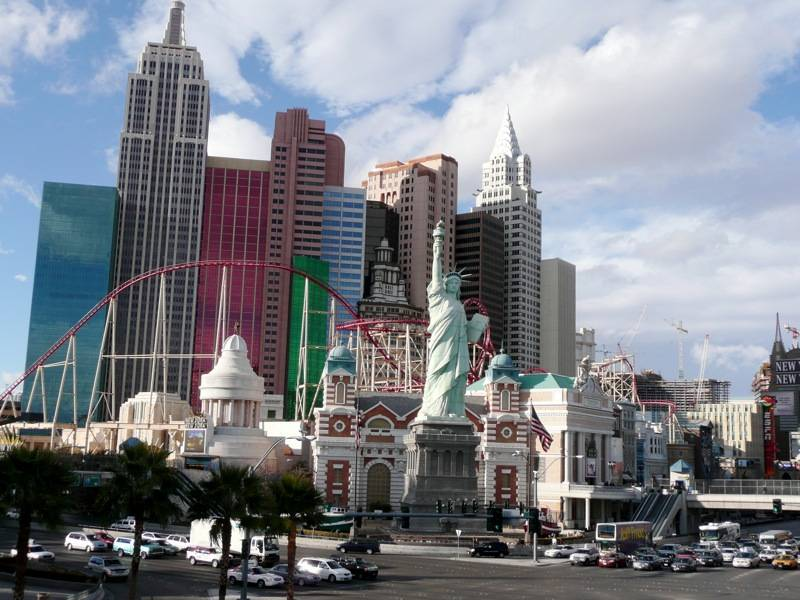
\includegraphics[width=\textwidth, keepaspectratio]{placeholder/800-600-1}
        \caption{Picture 1.}
        \label{fig:subfigures-four:1}
    \end{subfigure}
    \hfill
    \begin{subfigure}[b]{0.49\textwidth}
        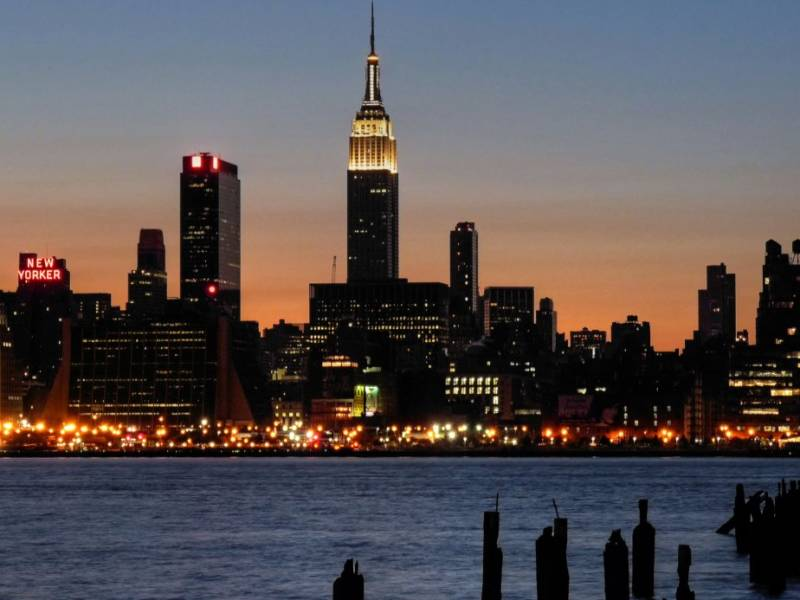
\includegraphics[width=\textwidth, keepaspectratio]{placeholder/800-600-2}
        \caption{Picture 2.}
        \label{fig:subfigures-four:2}
    \end{subfigure}
    \hfill
    \begin{subfigure}[b]{0.49\textwidth}
        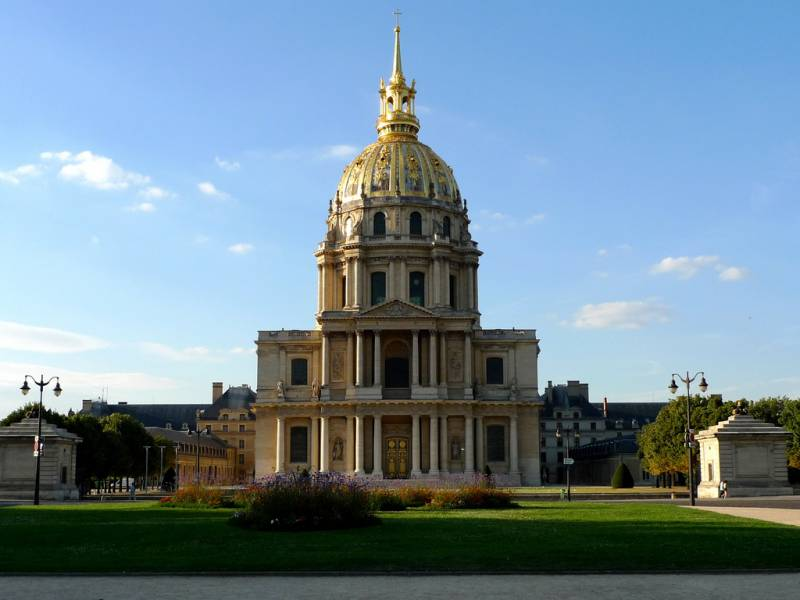
\includegraphics[width=\textwidth, keepaspectratio]{placeholder/800-600-3}
        \caption{Picture 3.}
        \label{fig:subfigures-four:3}
    \end{subfigure}
    \hfill
    \begin{subfigure}[b]{0.49\textwidth}
        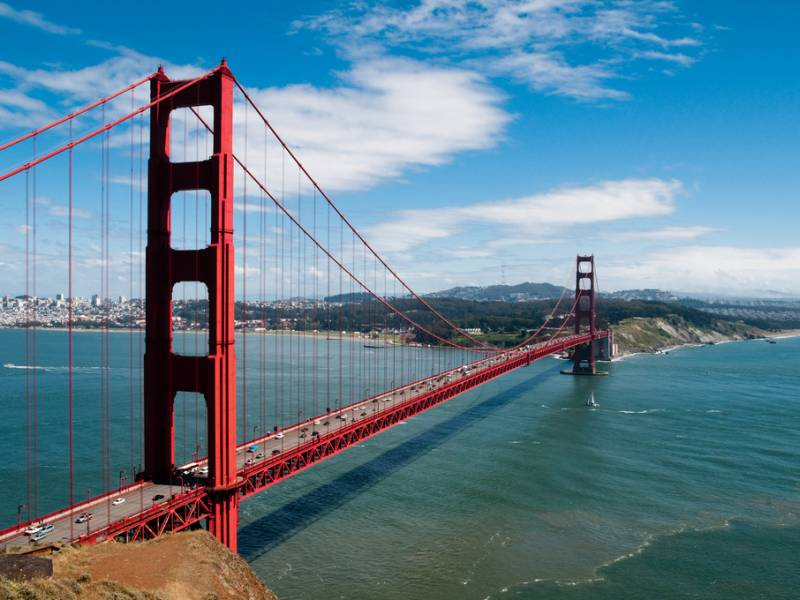
\includegraphics[width=\textwidth, keepaspectratio]{placeholder/800-600-4}
        \caption{Picture 4.}
        \label{fig:subfigures-four:4}
    \end{subfigure}
    
    \caption{Even subfigures of four figures are possible.}
    \label{fig:subfigures-four}
\end{figure}

\begin{table}
    \centering
    \caption{A sample table}
    \label{tbl:sample-table}
    \begin{tabular}{@{}llr@{}} \toprule
        \multicolumn{2}{c}{Item} \\ \cmidrule(r){1-2}
        Animal & Description & Price (\$)\\ \midrule
        Gnat  & per gram  & 13.65 \\
        & each      & 0.01 \\
        Gnu   & stuffed   & 92.50 \\
        Emu   & stuffed   & 33.33 \\
        Armadillo & frozen & 8.99 \\ \bottomrule
    \end{tabular}
\end{table}

\begin{table}
    \centering
    \caption{Tables can look nice, even for many many data to display}
    \label{tbl:sample-table-large}
    \begin{tabular}{SSSSSSSS} \toprule
        {$m$} & {$\Re\{\underline{\mathfrak{X}}(m)\}$} & {$-\Im\{\underline{\mathfrak{X}}(m)\}$} & {$\mathfrak{X}(m)$} & {$\frac{\mathfrak{X}(m)}{23}$} & {$A_m$} & {$\varphi(m)\ /\ ^{\circ}$} & {$\varphi_m\ /\ ^{\circ}$} \\ \midrule
        1  & 16.128 & +8.872 & 16.128 & 1.402 & 1.373 & -146.6 & -137.6 \\
        2  & 3.442  & -2.509 & 3.442  & 0.299 & 0.343 & 133.2  & 152.4  \\
        3  & 1.826  & -0.363 & 1.826  & 0.159 & 0.119 & 168.5  & -161.1 \\
        4  & 0.993  & -0.429 & 0.993  & 0.086 & 0.08  & 25.6   & 90     \\ \midrule
        5  & 1.29   & +0.099 & 1.29   & 0.112 & 0.097 & -175.6 & -114.7 \\
        6  & 0.483  & -0.183 & 0.483  & 0.042 & 0.063 & 22.3   & 122.5  \\
        7  & 0.766  & -0.475 & 0.766  & 0.067 & 0.039 & 141.6  & -122   \\
        8  & 0.624  & +0.365 & 0.624  & 0.054 & 0.04  & -35.7  & 90     \\ \midrule
        9  & 0.641  & -0.466 & 0.641  & 0.056 & 0.045 & 133.3  & -106.3 \\
        10 & 0.45   & +0.421 & 0.45   & 0.039 & 0.034 & -69.4  & 110.9  \\
        11 & 0.598  & -0.597 & 0.598  & 0.052 & 0.025 & 92.3   & -109.3 \\ \bottomrule
    \end{tabular}
\end{table}

%    \begin{lstlisting}
%        \begin{minted}{latex}
%\begin{figure}
%    \centering
%    \includegraphics[width=\linewidth, keepaspectratio=true]%
%        {placeholder/14942249547_f7f1d3e8bd_k}
%    \caption{A sample figure to show the effect of a loooong looooong caption. %
%        Credits by \url{https://www.flickr.com/photos/schubi74/14942249547/}.}
%    \label{fig:sample-figure}
%\end{figure}
%        \end{minted}
%        \caption{Sample code for \cref{fig:sample-figure}}
%        \label{lst:sample-code}
%    \end{lstlisting}

For figures, the guidelines are:

\begin{itemize}
    \item Always center images using \verb|\centering| as the very first command of the \verb|figure|-environment.
    \item Make sure to set the width of your included images explicitely using the \verb|width=| option. Have a single figure's width set to \verb|width=0.75\linewidth|, while two figures side by side must be set to \verb|width=\linewidth| as long as you set the width of the surrounding \verb|minipage| or \verb|subfigure| to \verb|0.49\linewidth|
    \item Don't forget to keep the aspect ratio of images if you change their width.
    \item Never ever under sample images. In other words: never ever enlarge images.
    \item It's best to use vector graphics i.e., \verb|*.eps| or \verb|*.tikz| for proper quality in both PDFs as well as on screen.
    \item Add a caption to your image. Captions must be below the image.
    \item Let the labels be handled automatically by \LaTeX. A best practice is to set the prefix of figures' labels to \verb|fig:|.
    \item For a good example see \cref{fig:sample-figure} and its code at \cref{lst:sample-code} (this reference was created using the \verb|\cref{}| command).
    \item Always add a full stop to your figure captions like so.
    \item Do not be afraid to use lengthy figure and table captions—better that than confusing or incomplete ones.
    \item If your figure or table is essentially the same as or based on another author’s, but you recreated or adapted it, it is standard to include the words “Adapted from” or “After” followed by the author’s name and a citation at the end of the caption.
    \item Always cite the figure or table if it—--or its data—--came from a source, using the same citation style that you have used throughout the paper. The most logical place for the citation to appear is at the end of the caption. See \cref{sec:referencing} of this manual for a thorough discussion of rules for source citation.
    \item Do not crowd a table or figure, neither within itself nor within your text; give it room to breathe. When it appears amidst your body text, skip at least one line above and below it.
    \item Rule of thumb: Try to present the table or figure so that it would make sense even if ripped from the paper.
    \item If possible, label the axes of graphs with full words: ``Temperature versus time'' rather than ``T versus t.''
    \item Be certain that your legend—--that part of the figure where you define any symbols or other visual markers that appear—--is readable, clear, and meaningfully placed. As long as it does not overwhelm the rest of the figure, do not be afraid to make the legend large to enhance its readability.
    \item Use footnotes (a simple asterisk to indicate them will do) for explanatory material such as the number of respondents to a survey or the fact that certain values were estimated.
\end{itemize}

For tables, the guidelines are

\begin{itemize}
    \item The legend (sometimes called the caption) goes above the Table.
    \item Units are specified in column headings wherever appropriate.
    \item Lines of demarcation are used to set legend, headers, data, and footnotes apart from one another.
    \item Footnotes are used to clarify points in the table, or to convey repetitive information about entries.
    \item Footnotes may also be used to denote statistical differences among groups.
\end{itemize}


\section{Coloring}

There are a few basic colors that are set for some default coloring of tables and should be used primarily for other things, where applicable.

\begin{itemize}
    \item very light gray \textcolor{VLGray}{VLGray}
    \item light gray \textcolor{LGray}{LGray}
    \item medium gray \textcolor{MGray}{MGray}
    \item dark gray \textcolor{DGray}{DGray}
    \item vary dark gray \textcolor{VDGray}{VDGray}
    \item very very dark gray \textcolor{VVDGray}{VVDGray}
\end{itemize}


\section{Referencing}\label{sec:referencing}

Referencing may be done using \verb|\ref{label}| even though usage of \verb|\cref{label}| is encouraged for that it automatically typesets the appropriate type like \texttt{Eqn.} or \texttt{Fig.}, \texttt{Tbl.}, or \texttt{Listing} to whatever is being reference. At the beginning of a sentence, \verb|\Cref{label}| must be used to fully give the referenced type in words. \Cref{fig:sample-figure} refers to a sample figure at the beginning of a sentence, while \cref{fig:sample-figure} refers to a sample figure in text.

\begin{itemize}
    \item Capitalise and write in words the reference object at the beginning of a sentence
    \item Otherwise use the abbreviated forms of \texttt{Fig.}, \texttt{Eqn.}, and \texttt{Tbl.} for referencing figures, equations, and tables, respectively
    \item Refer to the \verb|cleveref| package documentation at \\\url{http://www.ctan.org/pkg/cleveref}
\end{itemize}
